
\subsection{Convolutional Autoencoder with LSTM}
The CNN-AE-LSTM model is only the best performing model for one dataset, dataset 1.
Here the CNN-AE-LSTM local multivariate model structure beat the plain local multivariate LSTM with $1.09\%$.
The CNN-AE-LSTM performs competitively on all the experiments on dataset 1 except for the global univariate model structure.
Our experiments show that adding a Convolutional Autoencoder to an LSTM can be beneficial in some scenarios.


\begin{figure}[h!]
  \centering
  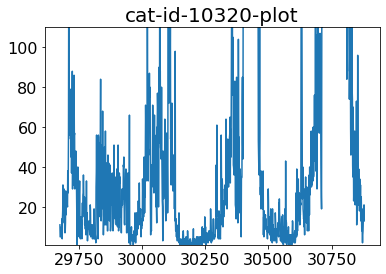
\includegraphics[width=\textwidth]{./figs/code_generated/data_exploration/cat-id-10320-plot.png}
  \hfill
  \caption{TODO}
  \label{fig:cat-id-10320-cnn-ae-beat-lstm}
\end{figure}

\import{./tables/results/dataset_high_variance}{Average-metric-dataset-high-variance.tex}

\begin{figure}[h!]
  \centering
  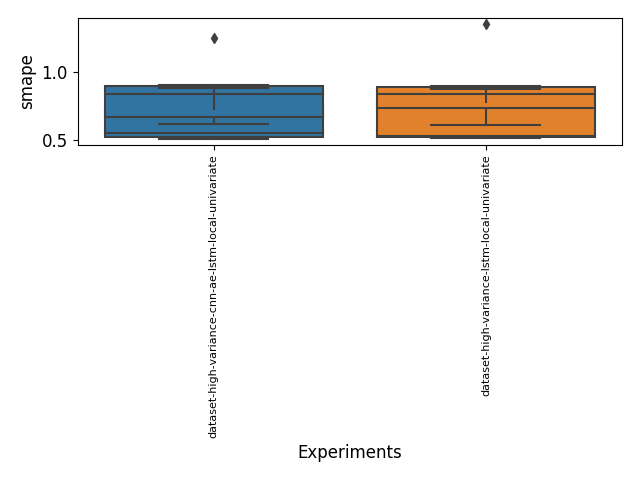
\includegraphics[width=\textwidth]{./figs/results/boxplot/smape-dataset_high_variance.png}
  \hfill
  \caption{TODO}
  \label{fig:results-smape-dataset-high-variance}
\end{figure}